\documentclass{beamer}
\usepackage[utf8]{inputenc}
\usepackage[french]{babel}
\usepackage[T1]{fontenc}
\usepackage{lmodern}
\usepackage{multirow}
\usepackage{multicol}
\usepackage[super]{nth}
%\usepackage{mlkkone}
\usepackage{hyperref}
\usepackage{MnSymbol,wasysym}
\usepackage{booktabs}
\usepackage{calc}
\usepackage{amssymb}
\usepackage{amstext}
\usepackage{amsmath}
\usepackage{amsthm}

\mode<presentation>{ %% on peut changer le style...
  \usetheme{Montpellier}
  \setbeamercovered{transparent}
  \setbeamertemplate{section in toc}[sections numbered]
  \setbeamertemplate{subsection in toc}[square]
}

\newcommand*\oldmacro{}%
\let\oldmacro\insertshorttitle%
\renewcommand*\insertshorttitle{%
  \oldmacro\hfill%
  \insertframenumber\,/\,\inserttotalframenumber}

\definecolor{links}{HTML}{2A1B81}
\hypersetup{colorlinks,linkcolor=,urlcolor=links,pdflang={francais}}
\author{Malik Koné\sup{1,2}, Madeth May\sup{1}, Sébastien Iksal\sup{1}, Souleyman Oumtanaga\sup{2}//\small{{\sup{1}LIUM, Le Mans Université, Le Mans, France}//\sup{2}LARIT, INP-HB, Yamoussoukro, Côte d'Ivoire}\url{\{malik.kone, madeth.may, sebastien.iksal\}@univ-lemans.fr}}

\date{\today}
\title{Towards visualizing collective dynamics in MOOC forums}
\hypersetup{
  pdfauthor={Malik Koné},
  pdftitle={},
  pdfkeywords={},
  pdfsubject={},
  pdfcreator={Emacs 26.1 (Org mode 9.1.9)},
  pdflang={English}}

%% première diapo en train d'être mise à jour
% \titlegraphic{\includegraphics[width=\textwidth]{./Images/logo_co}}  

\begin{document}
 %\frame{\titlepage}

\begin{frame}{Outline}
  \tableofcontents[hideallsubsections]
\end{frame}


\section{Context}

\begin{frame}{Section 1}
  \tableofcontents[sectionstyle=show/shaded,
  subsectionstyle=show/show/hide]
\end{frame}

\begin{frame}{Collective dynamics and visualisations}
  \only<0>{\cite{Baker2016,Dillenbourg2002,Tenenbaum2006,Vygotsky,Gerstenberg2017,Schwendimann2017,Twissel2014,Heer2012,Soller2005}}

  \only<0,1,2,3,4>{
    \begin{block}{Why visualize?}
      \begin{itemize}
      \item What are Learning dashboard and visualisations ? \tiny(Schwendimann2017) \normalsize

        \begin{itemize}
        \item Mirroring, metacognitiv, guiding and IA systems \tiny(Soller) \normalsize
        \item Over-scripting \tiny(Dillenbourg, 2002) \normalsize
        \item IA and stupid tutors \tiny (Baker, 2006) \normalsize
        \end{itemize}
        
      \item Help to make inferences \tiny (Twissell, 2014; Tenenbaum 2006, Heer 2012) \normalsize
      \item facilitate understanding via interactivity and exploration \tiny(Klerkx, 2014) \normalsize
      \item Challenges to model a theory or mind \tiny (gerstenberg, 2017) \normalsize
      \end{itemize}
    \end{block}
  }    

  \only<5->{
    \begin{columns}
      \begin{column}{.5\textwidth}
        \begin{block}{Why visualize?}
        \end{block}
        \begin{block}{What's collective dynamics?}
          \begin{itemize}
          \item An action: 
            \begin{itemize}
            \item Collective
            \item with temporal dynamics
            \item but also subjectiv
            \end{itemize}
          \end{itemize}
        \end{block}
      \end{column}

      \begin{column}{.5\textwidth}
        \includegraphics<6>[width=\textwidth]{./Images/processus}
        \includegraphics<7>[width=.7\textwidth]{./Images/dyn_vertical}
      \end{column}
    \end{columns}
  }

\end{frame}

\begin{frame}{Why visualising collective dynamics is important?}
  \only<1>{

    \begin{block}{Socio-construtivist reasons}
      \begin{itemize}
      \item discussion and human interactions => drive learners in their \emph{Proximal Developpement Zone}
      \end{itemize}
    \end{block}
    \begin{block}{Improve monitoring or learning}
    \end{block}
  }

\end{frame}

\section{Research question and hypothesis}

\begin{frame}{Section 2}
  \tableofcontents[sectionstyle=show/shaded,
  subsectionstyle=show/show/hide]
\end{frame}

\begin{frame}{How to measure collective dynamics?}
  \begin{itemize}
  \item Where to measure it?
  \item What to measure exactly?
  \end{itemize}
  
  \begin{block}{Technical hurdles?}
    \begin{itemize}
    \item Big data
    \item Reactivity
    \item Subjectivity of the collective dynamic
    \item NLP
    \end{itemize}
  \end{block}
\end{frame}

\begin{frame}{Hypothesis}
  \begin{itemize}
  \item We measure the collective dynamics in forum with:
    \begin{itemize}
    \item the temporal dimension
    \item the semantic dimension
    \item the structural (or social) dimension
    \end{itemize}
  \end{itemize}

  \begin{block}{but ... how should we combine indicators from those dimensions?}
  \end{block}
  
\end{frame}

\section{State of the art}

\begin{frame}{Section 3}
  \tableofcontents[sectionstyle=show/shaded,
  subsectionstyle=show/show/hide]
\end{frame}

\begin{frame}{Taking in account time, language and social dimension}
  \only<0>{\cite{Boroujeni2017}}
  \includegraphics<1>[width=\textwidth]{./Images/synthese1}
  \includegraphics<2>[width=\textwidth]{./Images/synthese2}
  \includegraphics<3>[width=\textwidth]{./Images/synthese3}
\end{frame}

\begin{frame}{Visualisation activities in Forums}
  \only<0>{\cite{Fu2017}}
  \only<1>{
    \centering 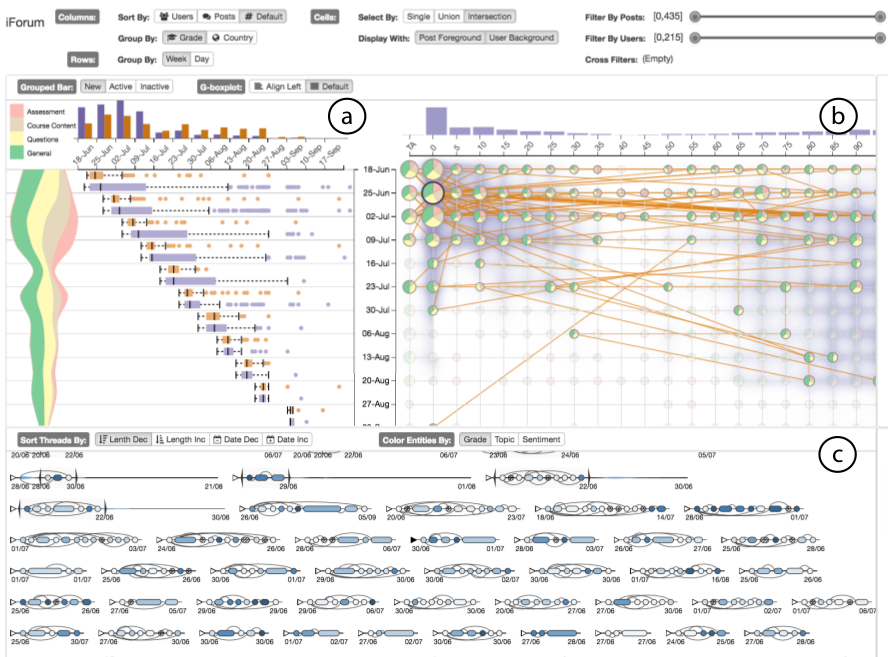
\includegraphics[width=.95\textwidth]{Images/fu.png}
    \tiny{Learning dashborad iForum (Fu 2017)}}
  \only<2>{
    \centering 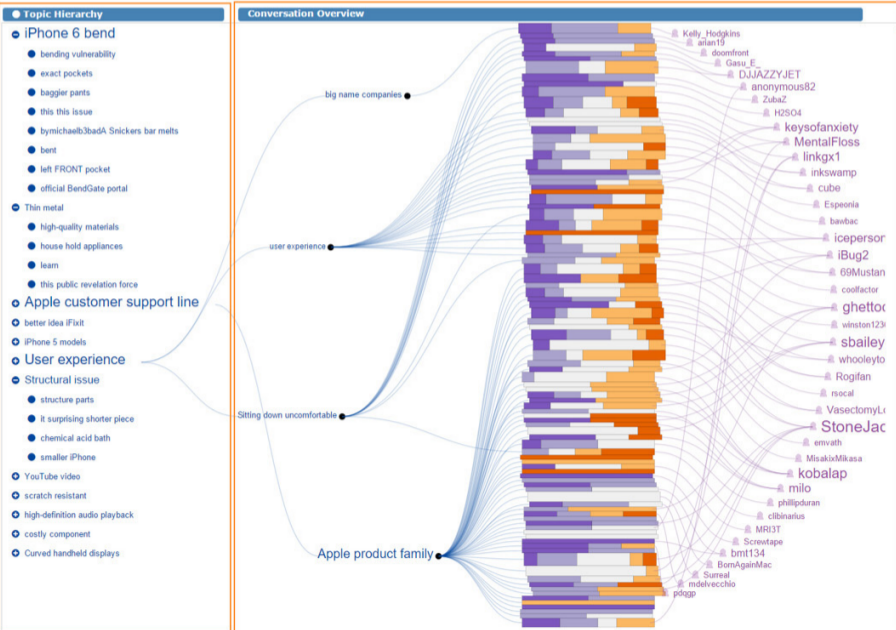
\includegraphics[width=.95\textwidth]{Images/convis.png}
    \tiny{Learning dashboard Convis (Hoque 2016) }}
\end{frame}

\section{Our contribution and results}

\begin{frame}{Section 4}
  \tableofcontents[sectionstyle=show/shaded,
  subsectionstyle=show/show/hide]
\end{frame}

\begin{frame}{We propose}
  \only<1>{
    \begin{block}{A method to collect and analyse collective actions}
      \centering 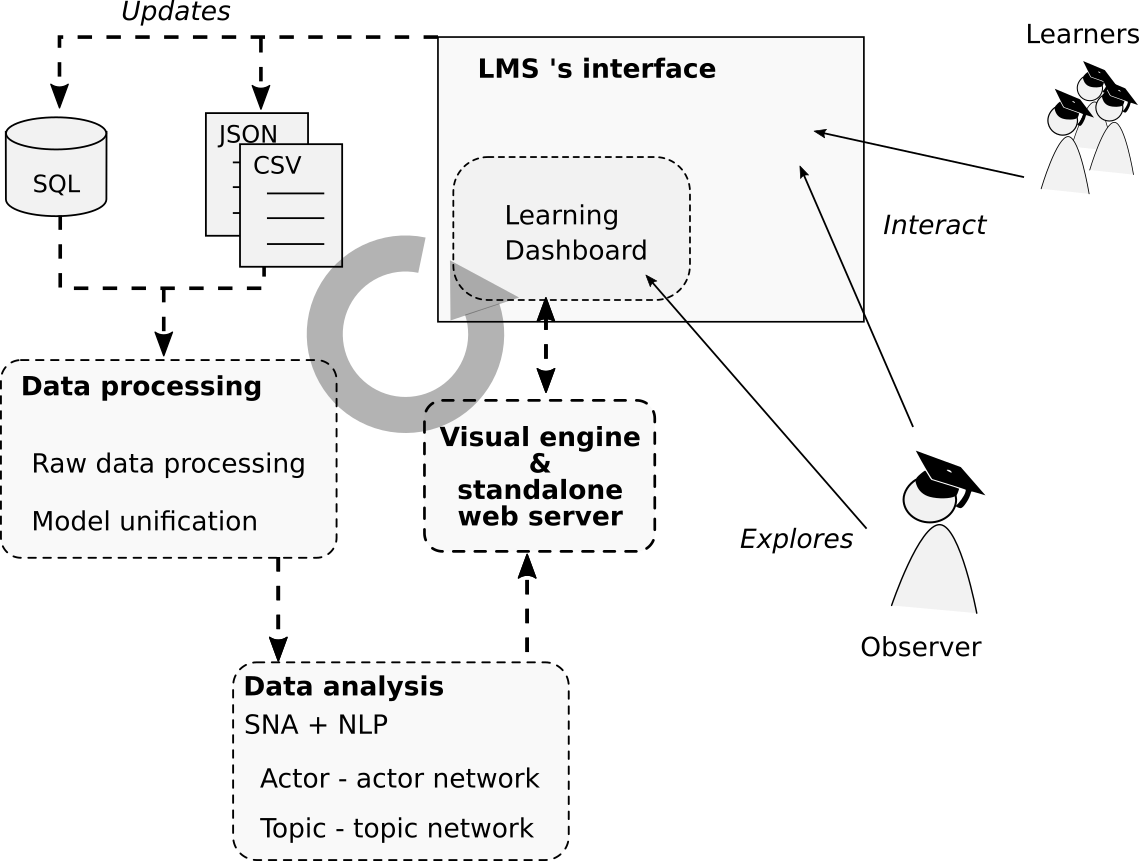
\includegraphics[width=.7\textwidth]{./Images/pipeline_en}  
    \end{block}
  }
  \only<2->{
    \begin{block}{A method to take in account the subjectif aspect of collective dynamics}
      \only<2>{
        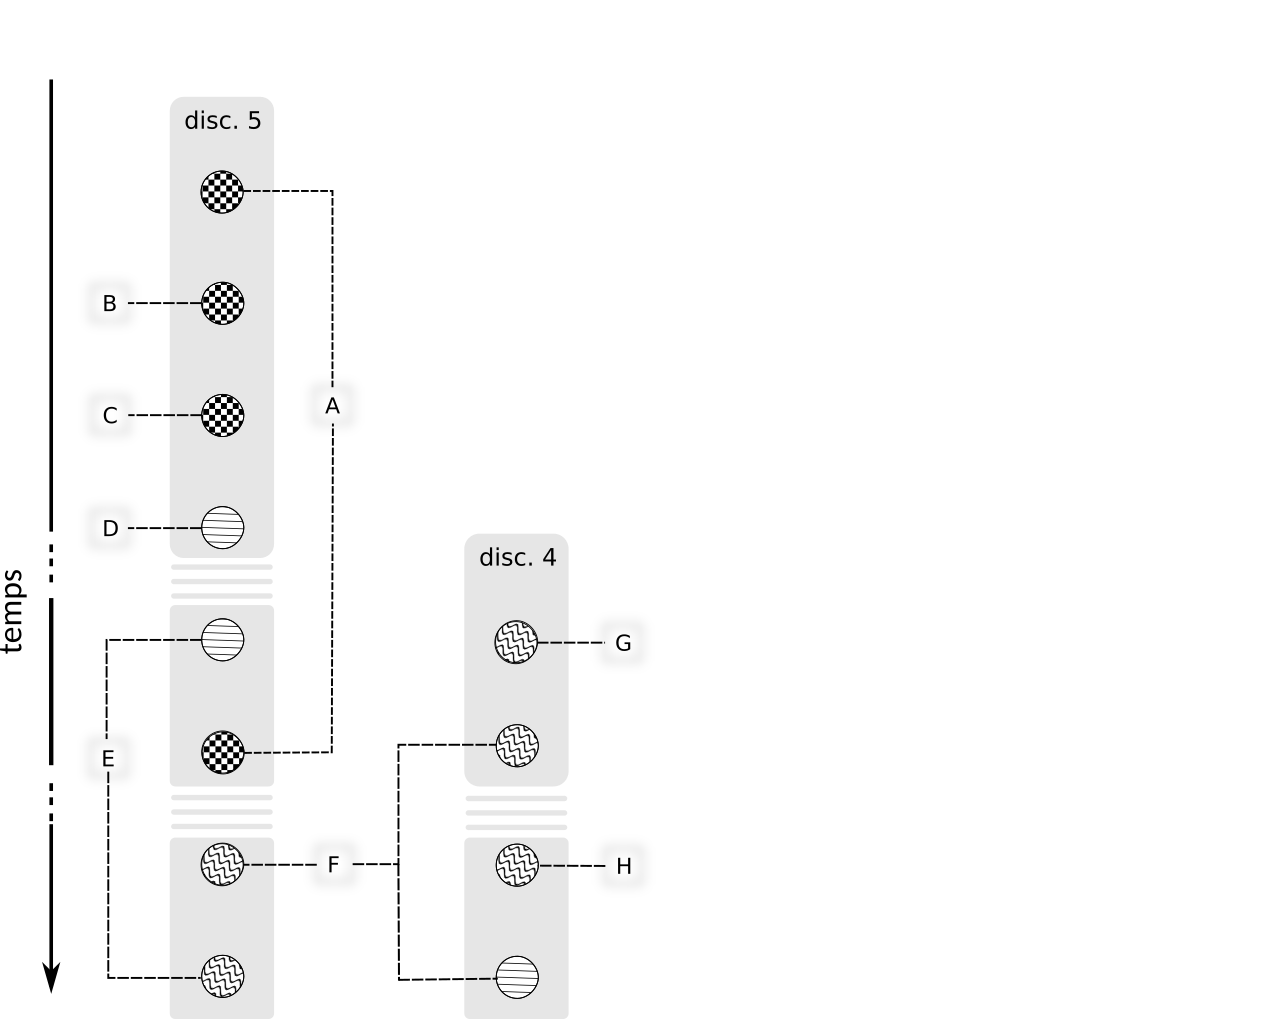
\includegraphics[width=.7\textwidth]{./Images/cycle0}
      }
      \only<3>{
        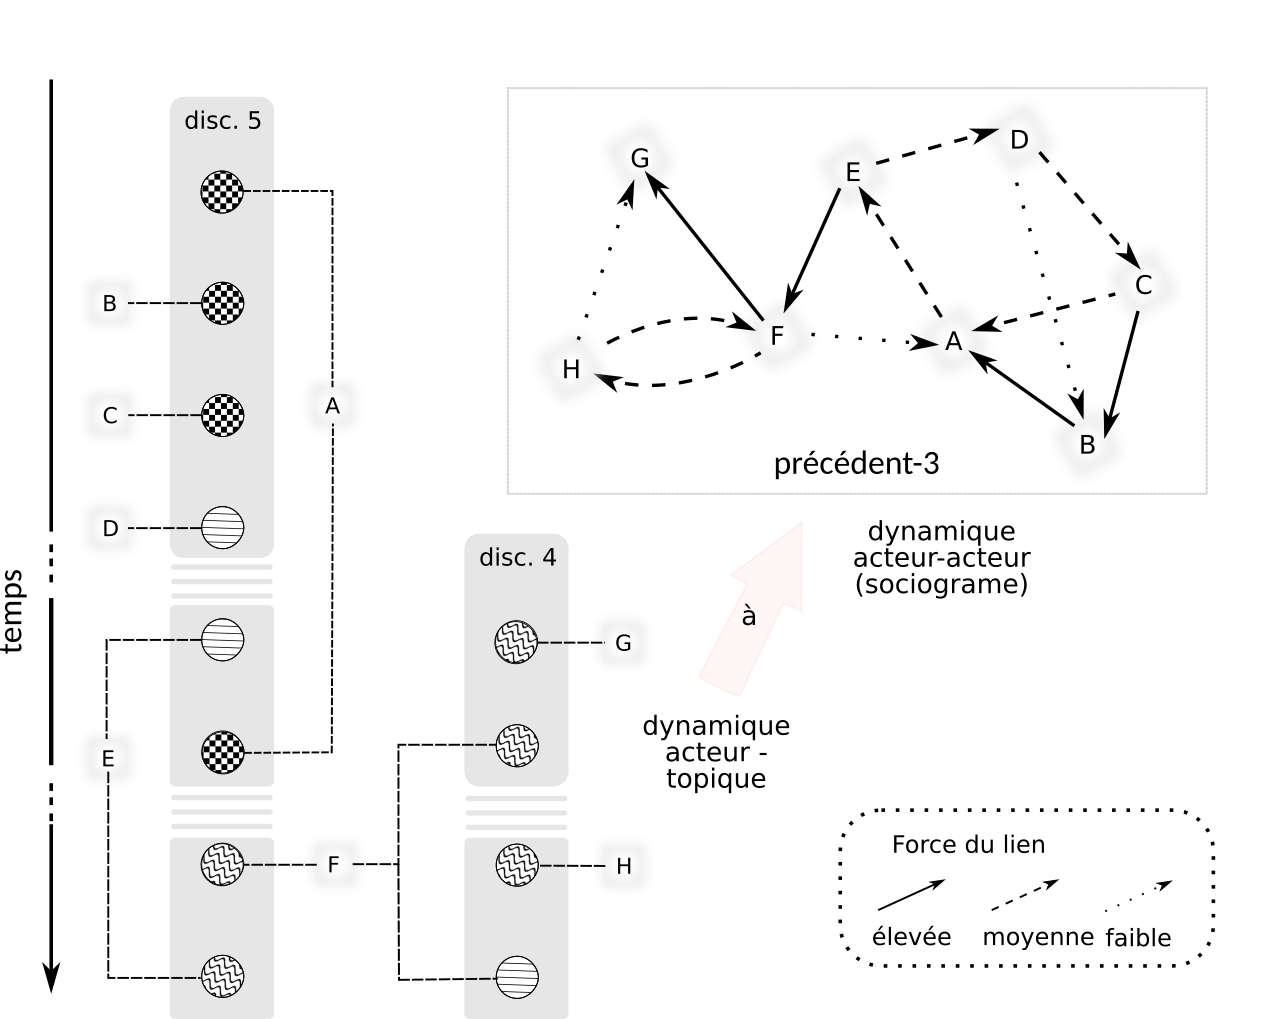
\includegraphics[width=.7\textwidth]{./Images/cycle1}
      }
      \only<4>{
        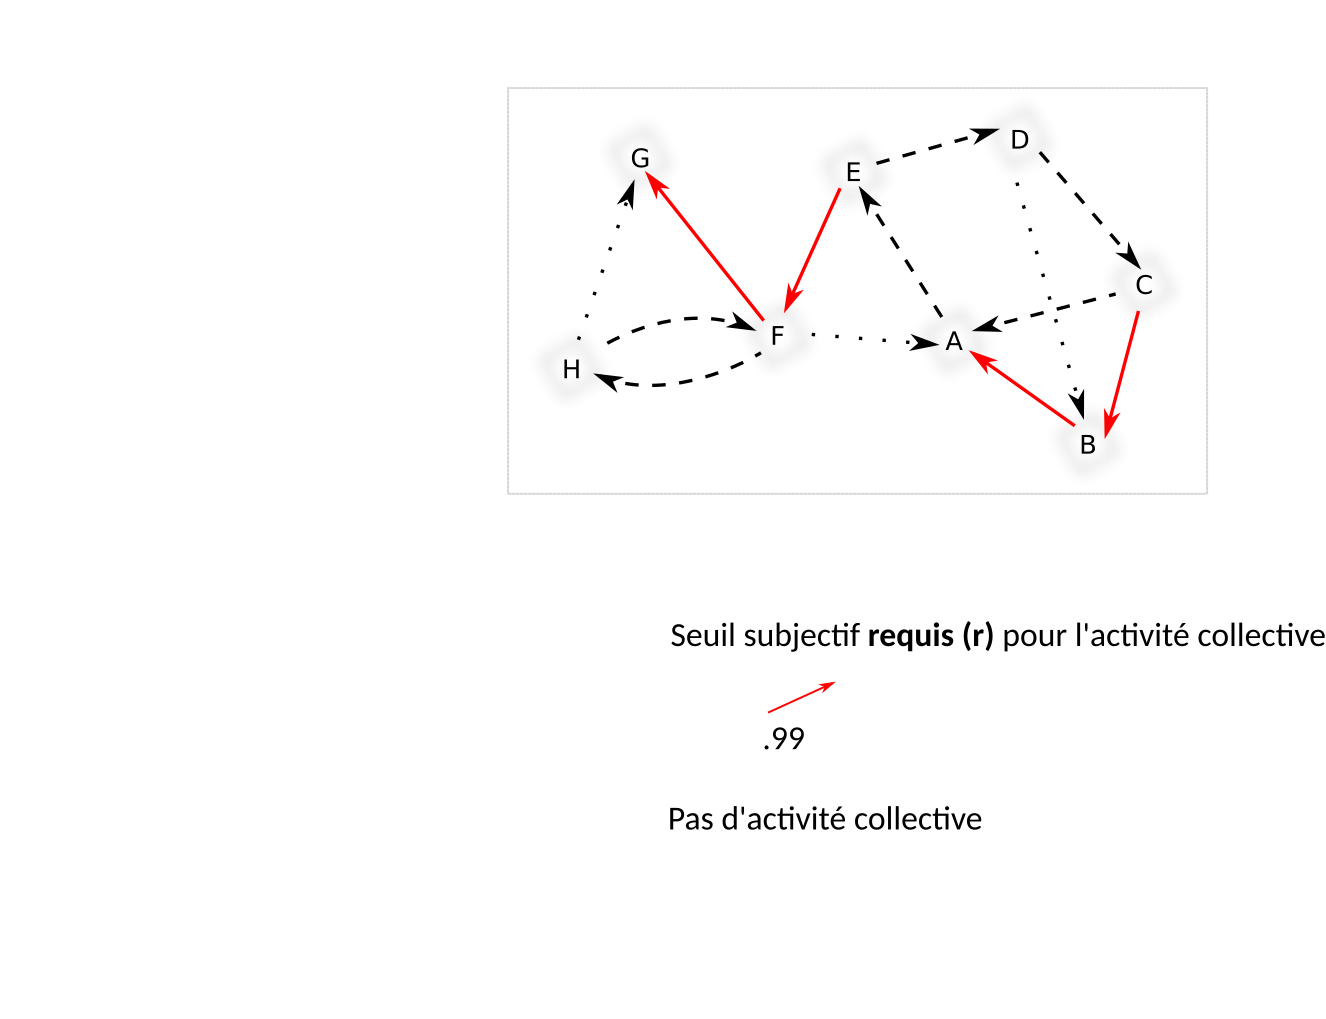
\includegraphics[width=.7\textwidth]{./Images/cycle2}
      }
      \only<5>{
        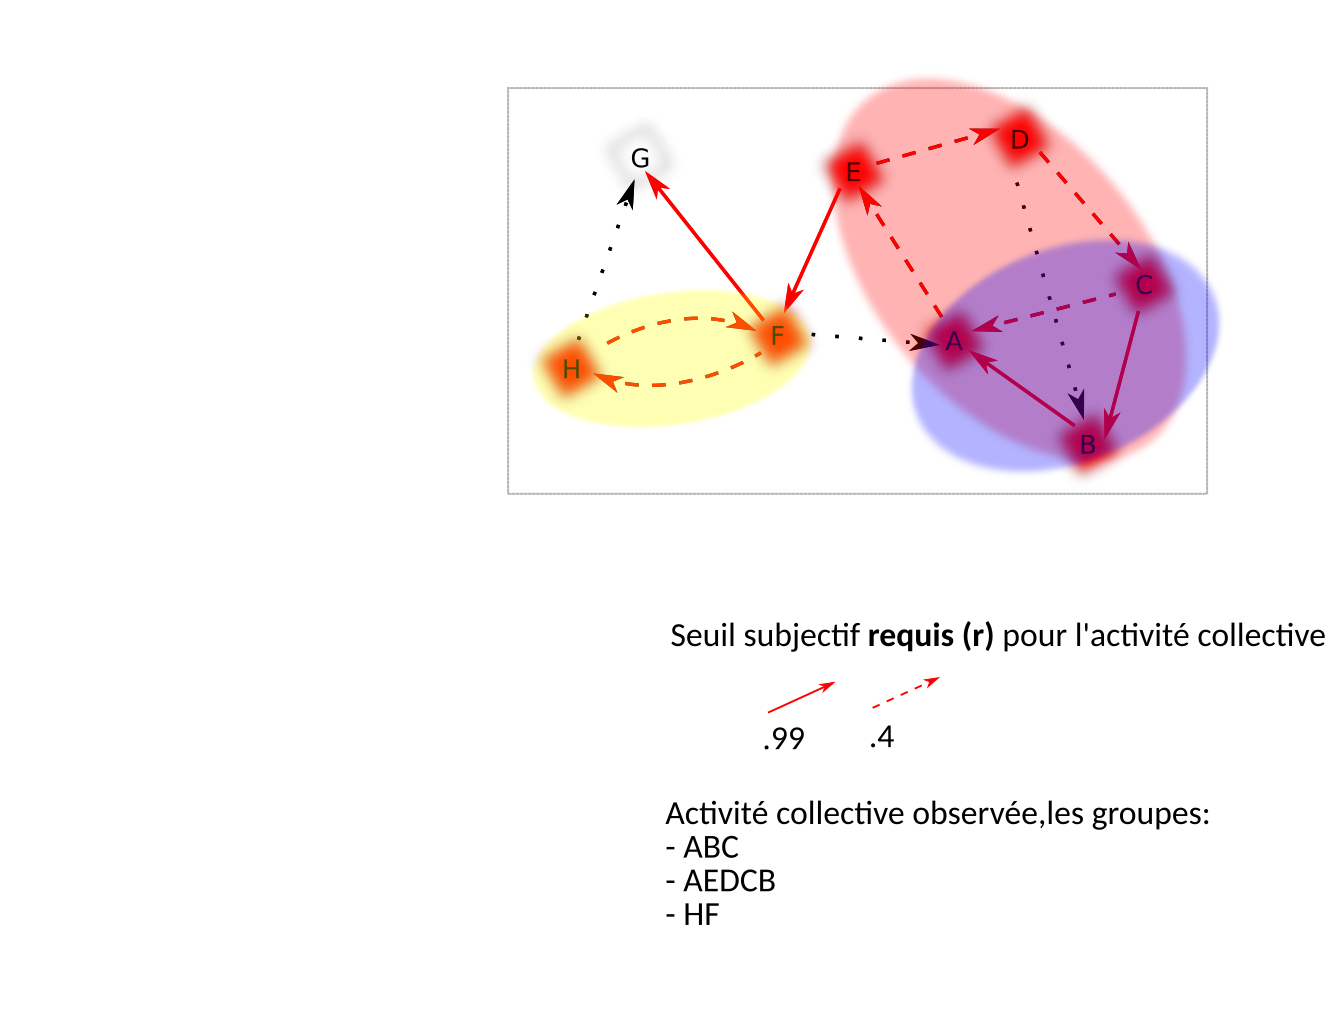
\includegraphics[width=.7\textwidth]{./Images/cycle3}
      }
      \only<6>{
        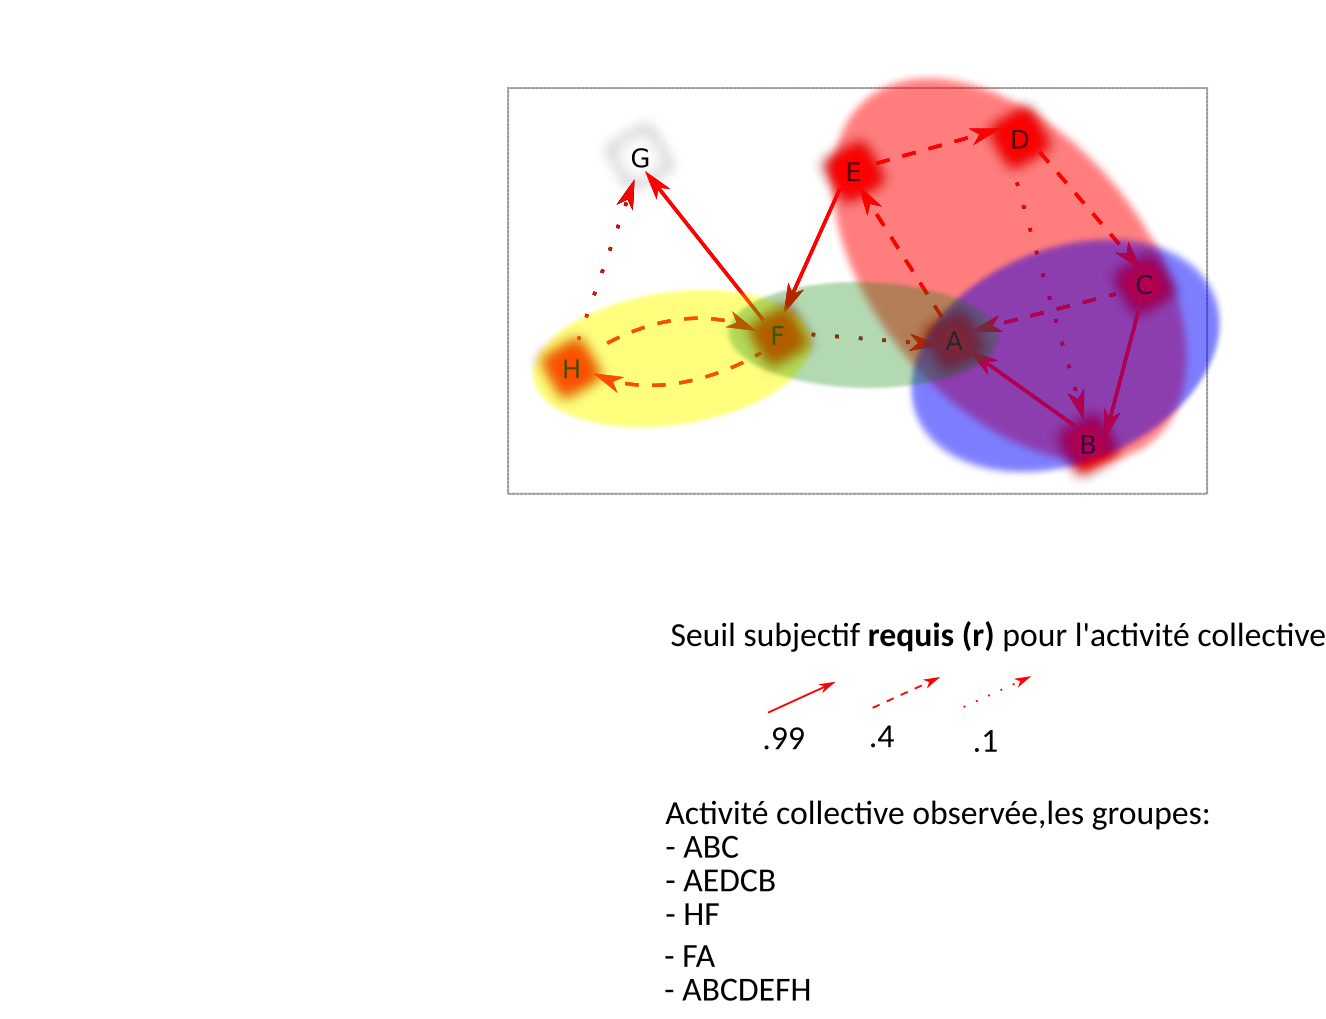
\includegraphics[width=.7\textwidth]{./Images/cycle4}
      }
      \only<7->{
        Here is an exemple of model for the interaction force

        \begin{columns}
          \begin{column}{.5\textwidth}
            \only<7>{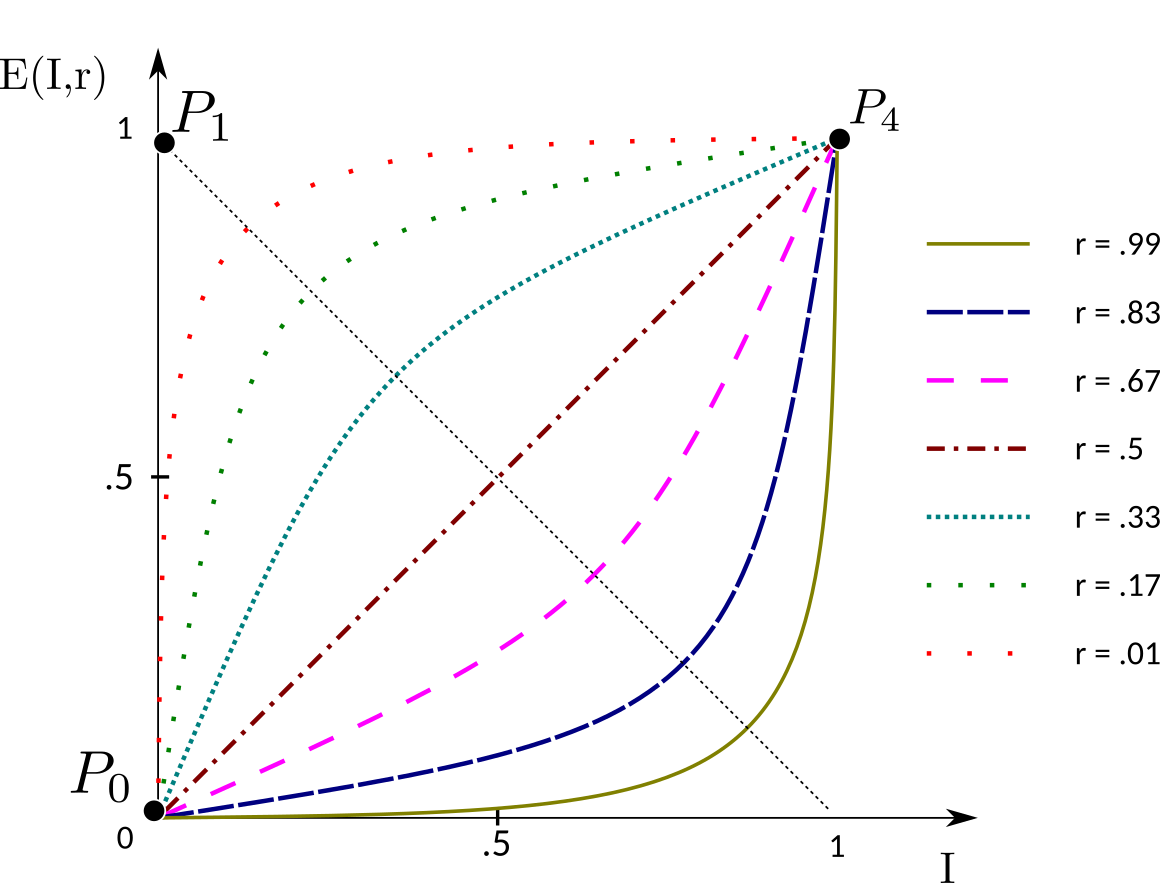
\includegraphics[width=\textwidth]{./Images/func2}}
            \only<8>{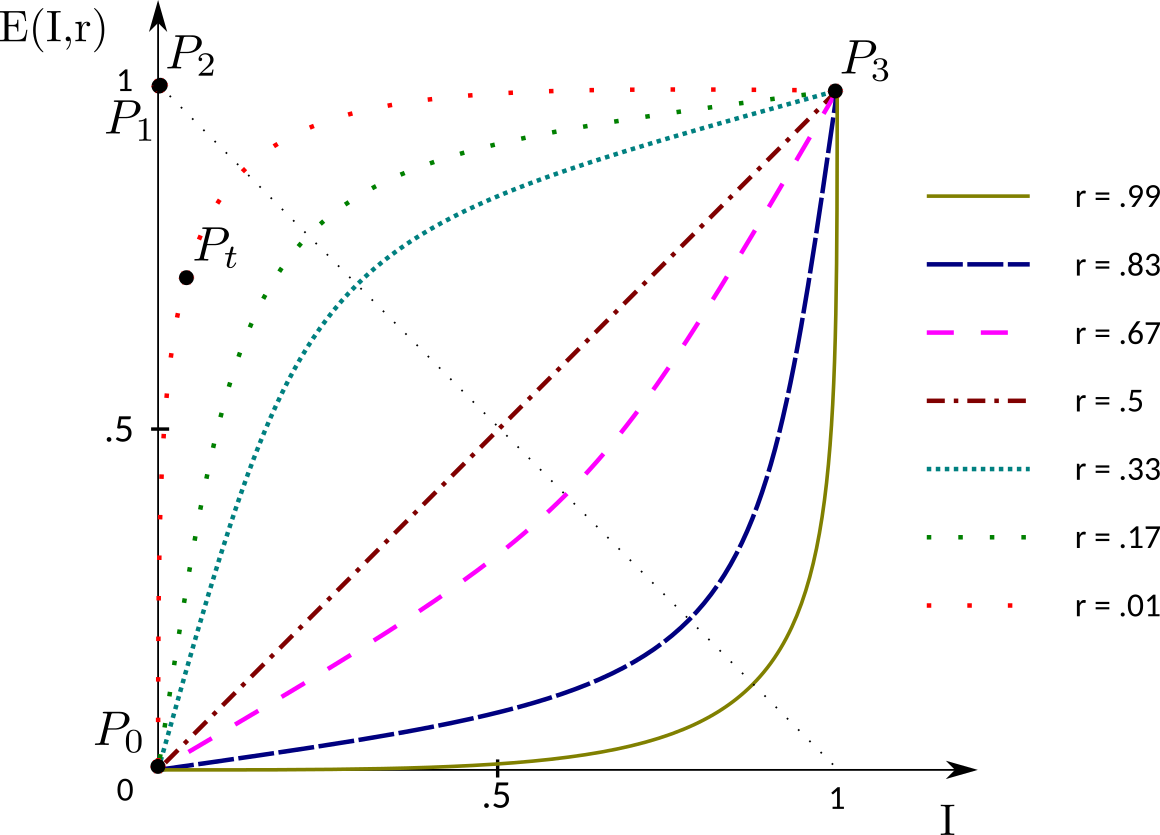
\includegraphics[width=\textwidth]{./Images/func2t1}}
            \only<9>{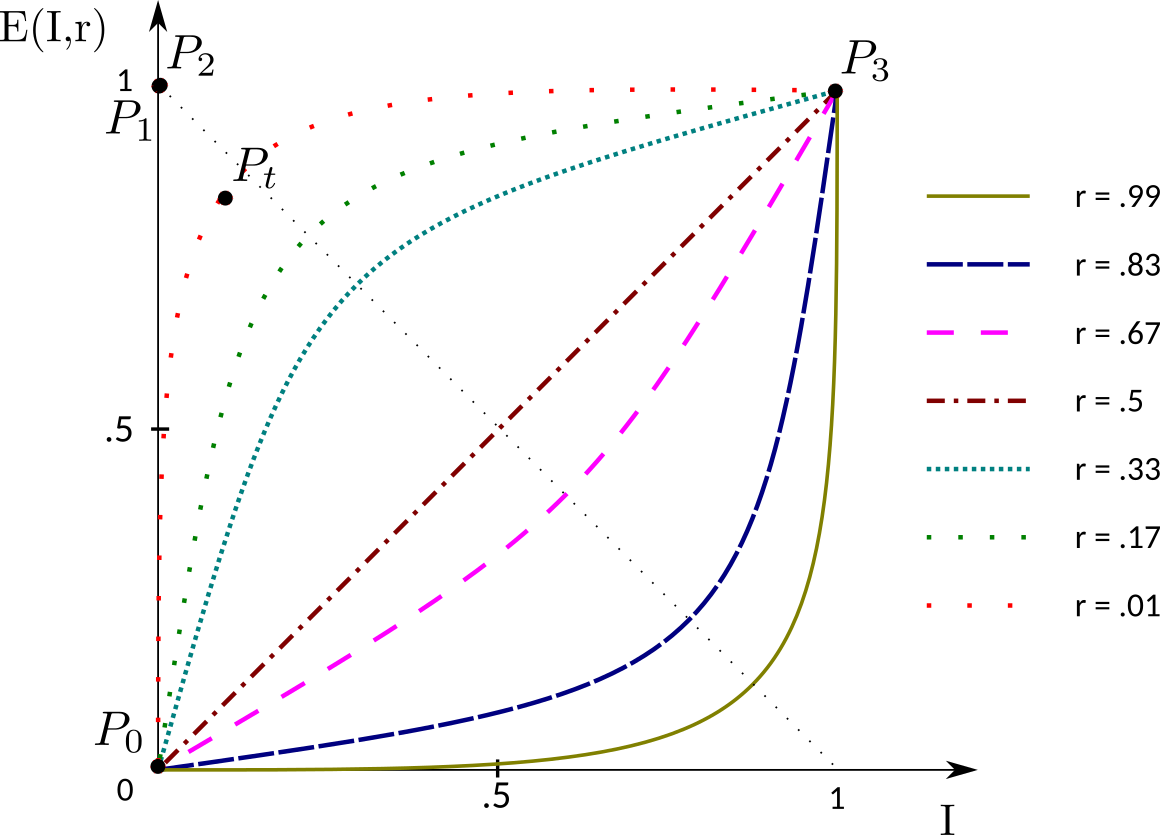
\includegraphics[width=\textwidth]{./Images/func2t2}}
            \only<10>{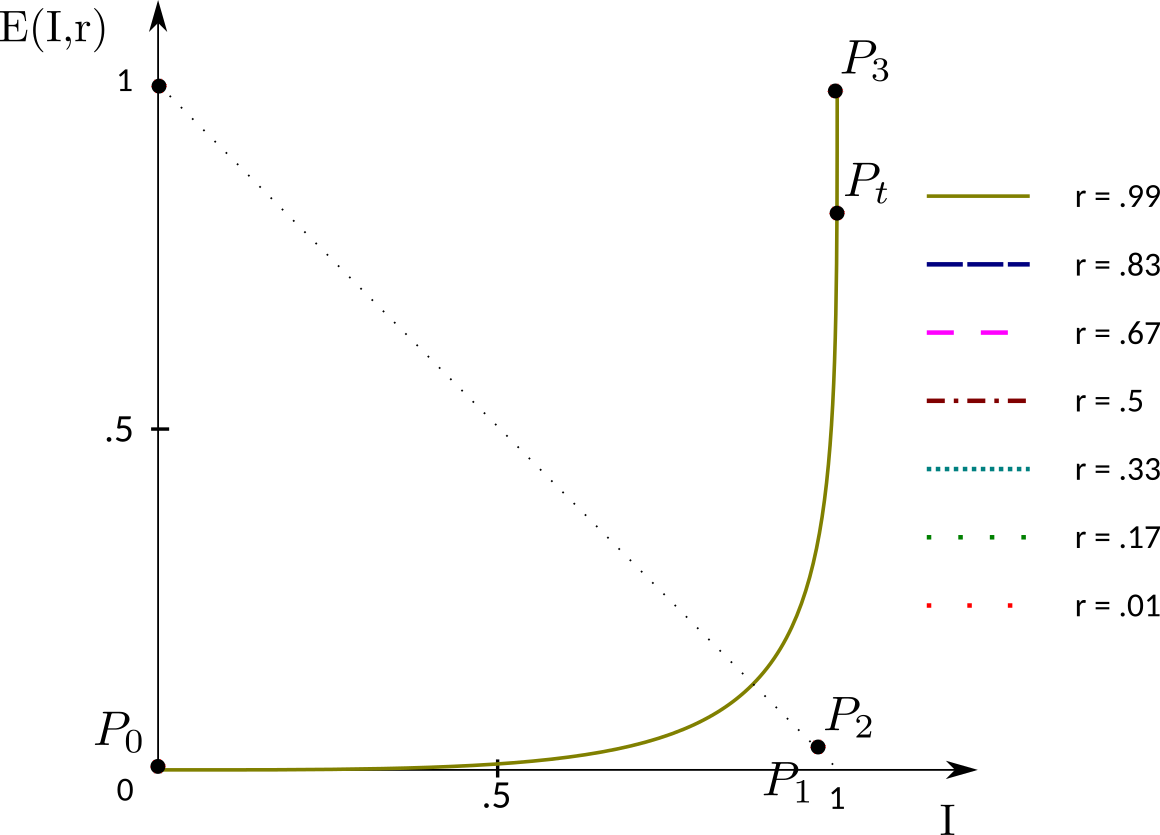
\includegraphics[width=\textwidth]{./Images/func2a}}
            \only<11>{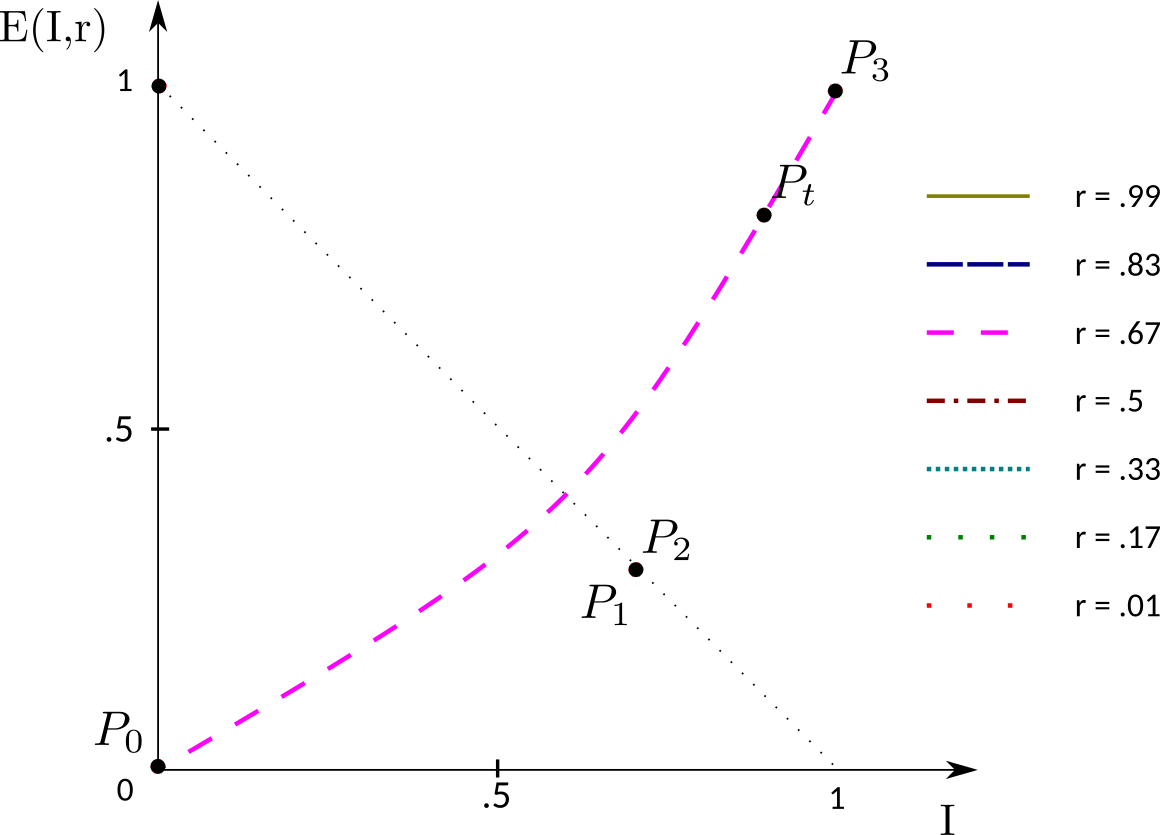
\includegraphics[width=\textwidth]{./Images/func2b}}
            \only<12>{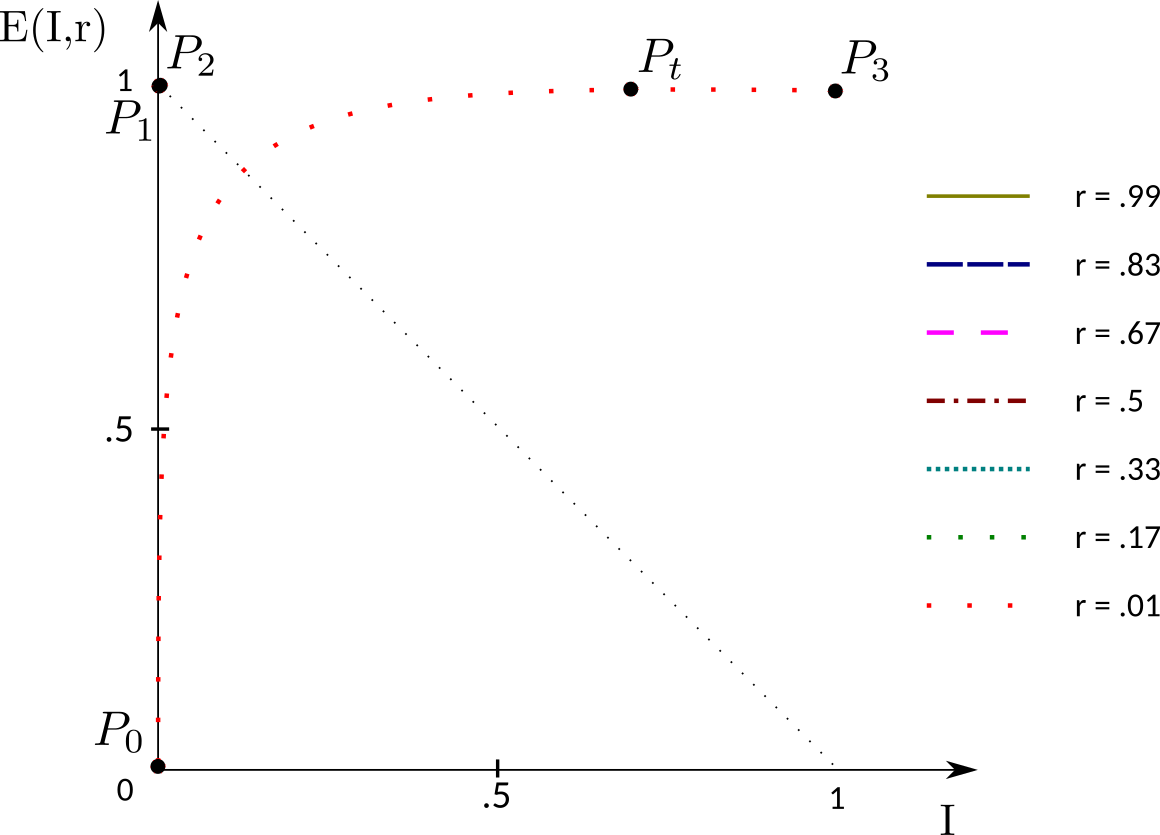
\includegraphics[width=\textwidth]{./Images/func2c}}
          \end{column}

          \begin{column}{.5\textwidth}
            \begin{align*}
              &P(t)=\sum_{i=0}^nB_{n,i}(t)P_i\\
              &\text{avec} \left \{
                \begin{aligned}
                  B_{n,i}(t)=\sum_{i=n}C_i^nt^i(1-t)^{n-i} \\
                  P_0=(0,0) \\
                  P_1=P_2=(0,1)\\
                  P_3=(1,1)\\
                  \text{et } t \in [0,1]
                \end{aligned} \right .
            \end{align*}
          \end{column}
        \end{columns}
      }
    \end{block}
  }

\end{frame}

\subsection{What did we look for?}

\begin{frame}{We looked for}
  \only<1>{

    \begin{block}{Existence of solution that could}
      \begin{itemize}
      \item Scale
      \item be reactice
      \item be multiplateform
      \end{itemize}
    \end{block}
  }
  \only<2,3>{
    \begin{block}{A solution that scale}
      \centering
      \only<2>{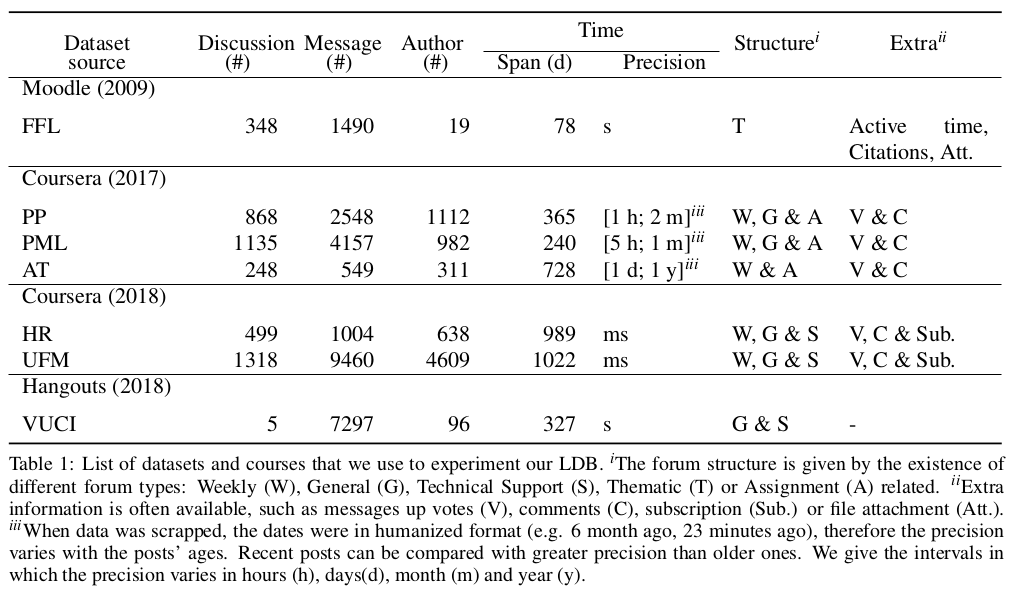
\includegraphics[width=.9\textwidth]{./Images/table}}
      \only<3>{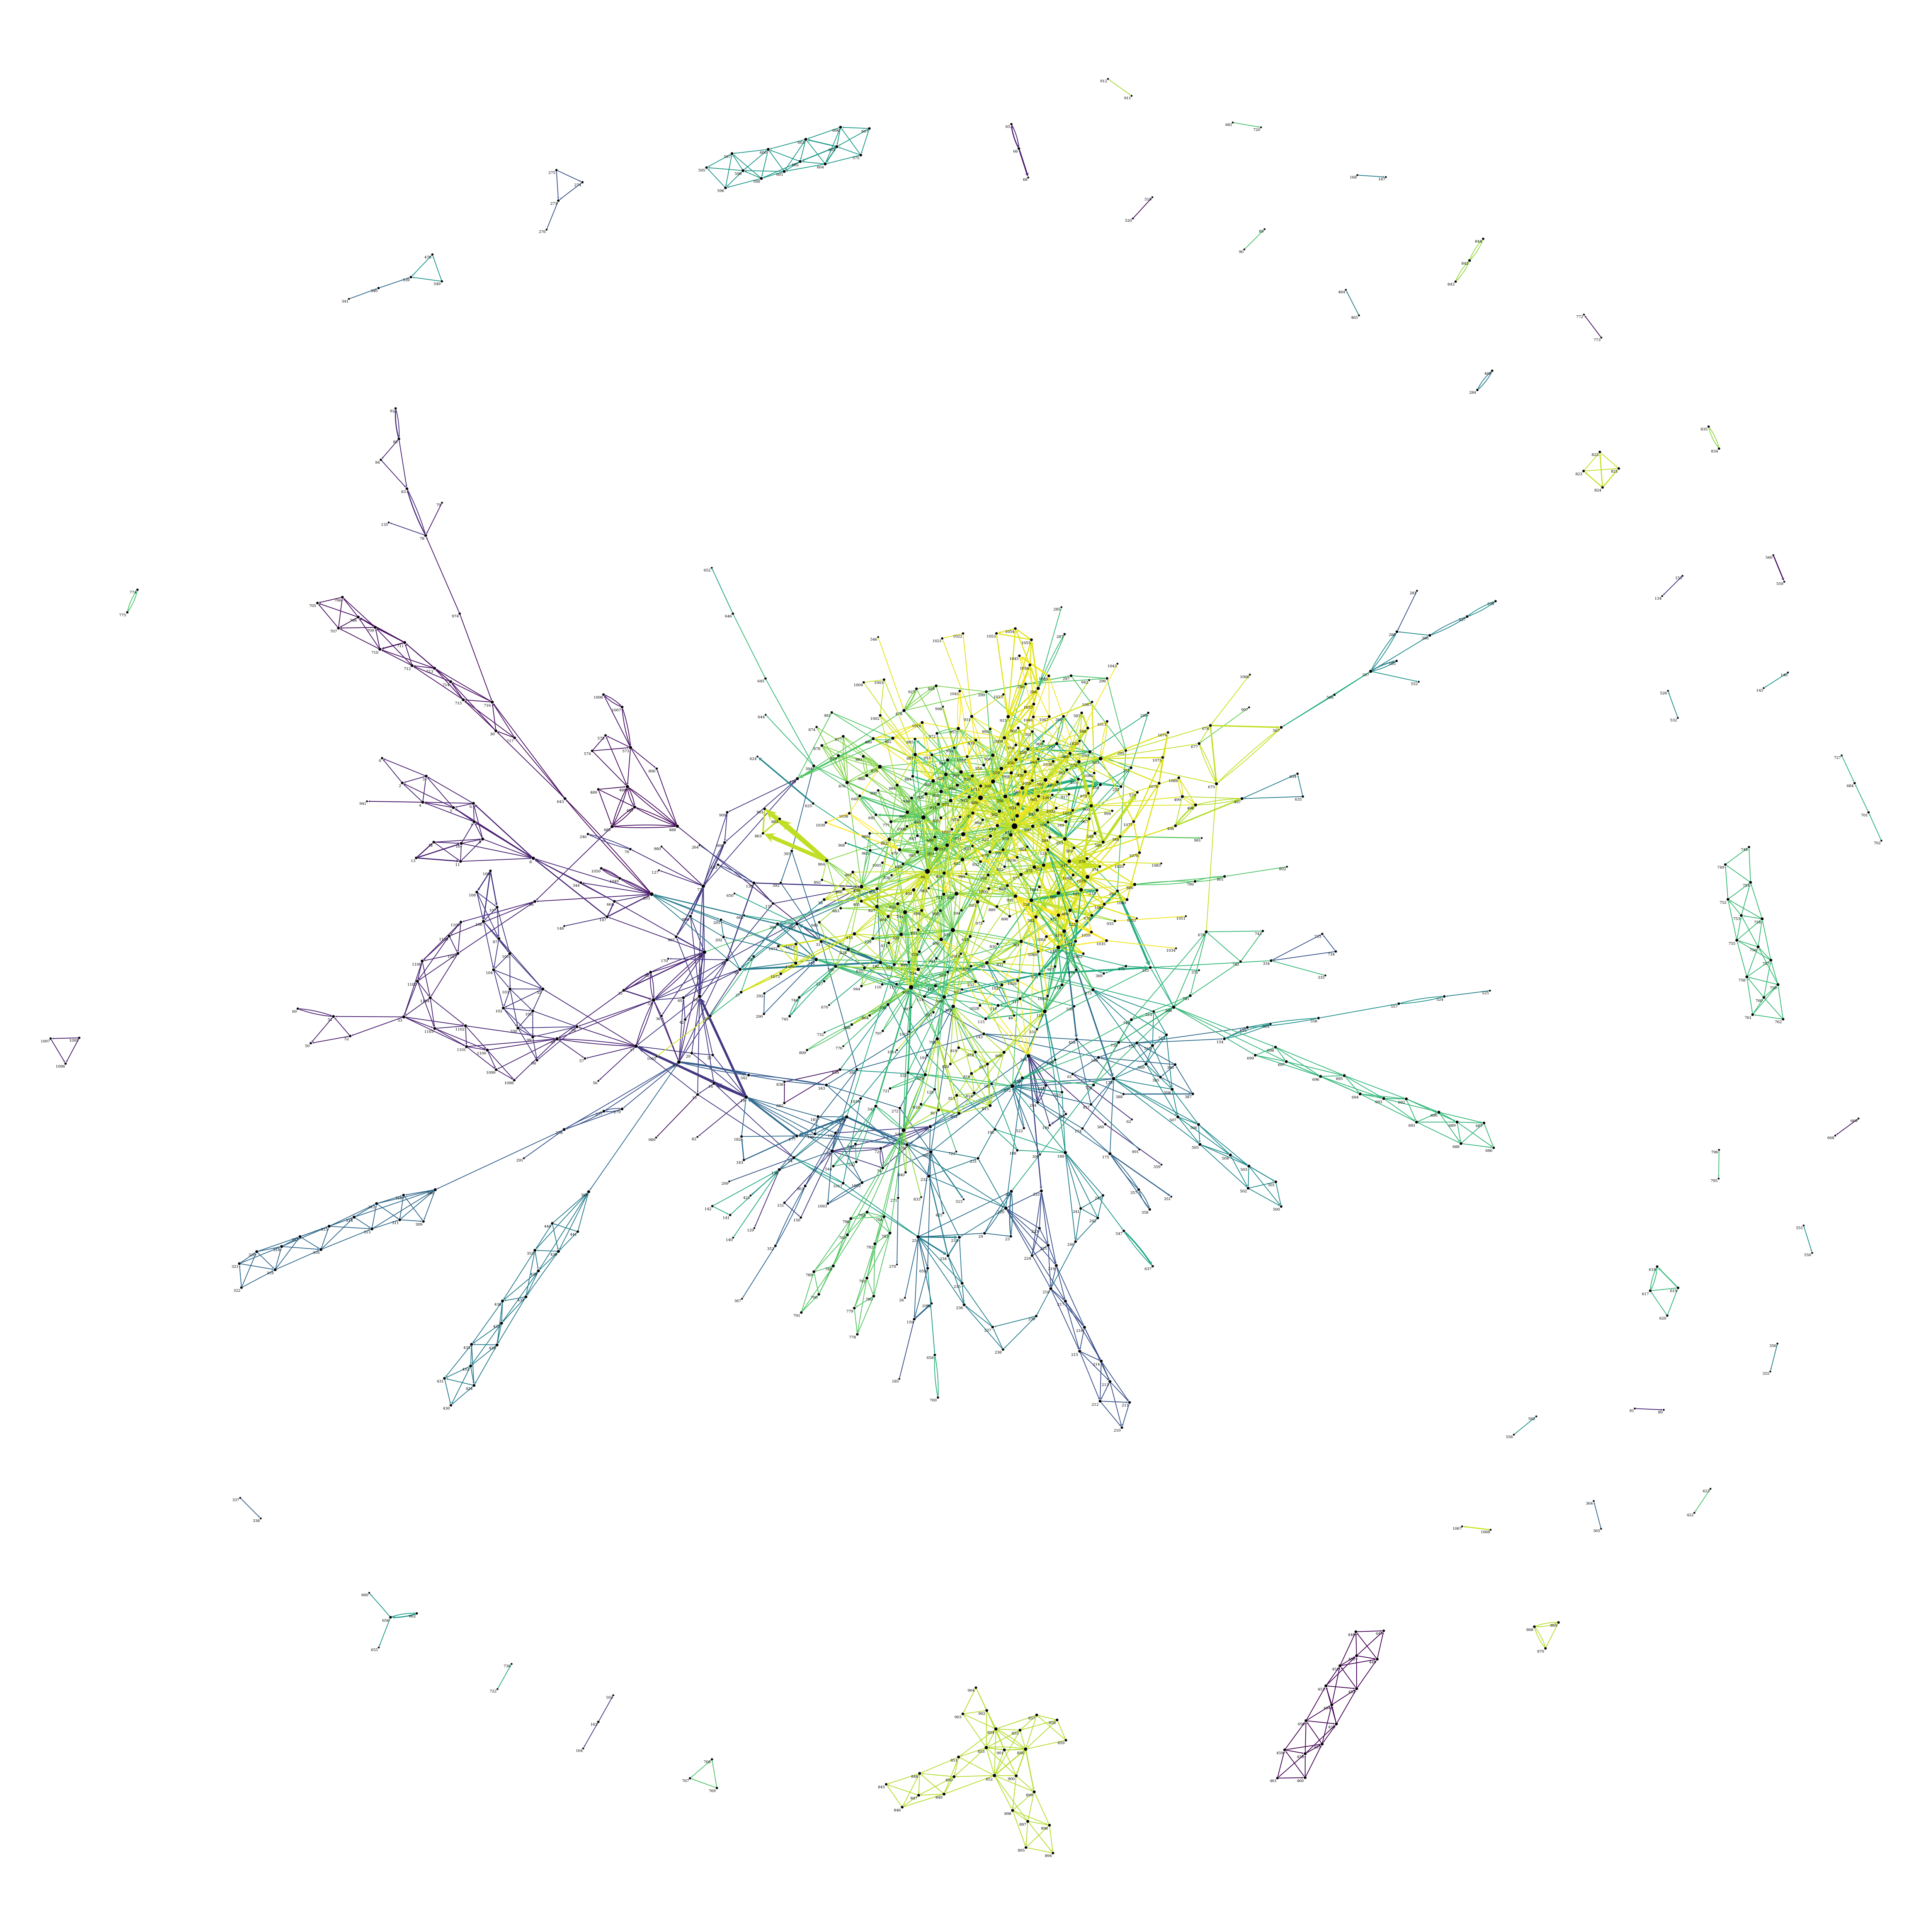
\includegraphics[width=.7\textwidth]{./Images/graphe}}
    \end{block}

  }
  \only<4,5>{
    \begin{block}{A reactive solution}
      \only<4>{\centering 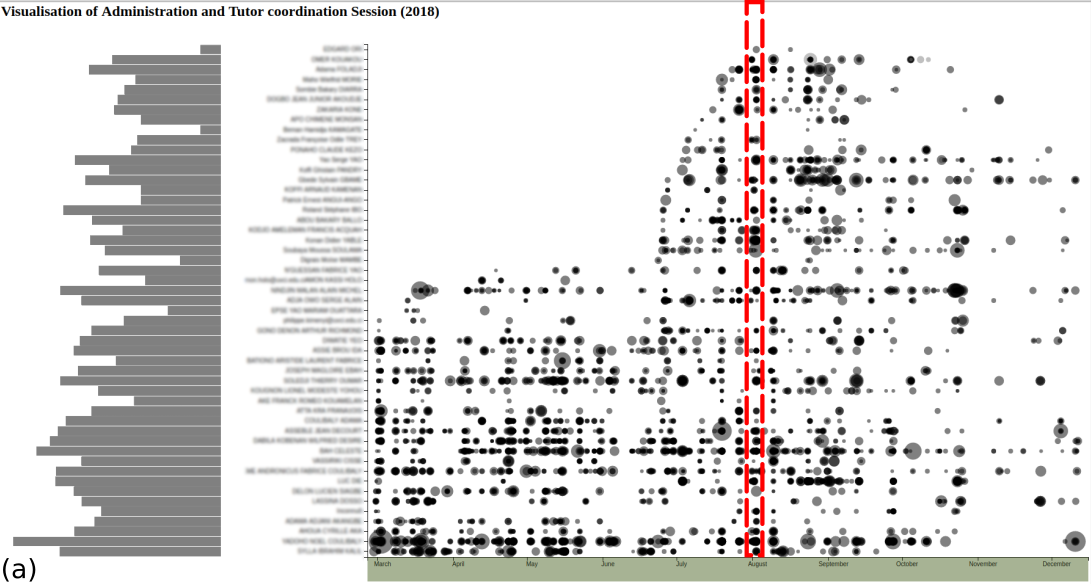
\includegraphics[width=.9\textwidth]{./Images/uvci_global}}
      \only<5>{\centering 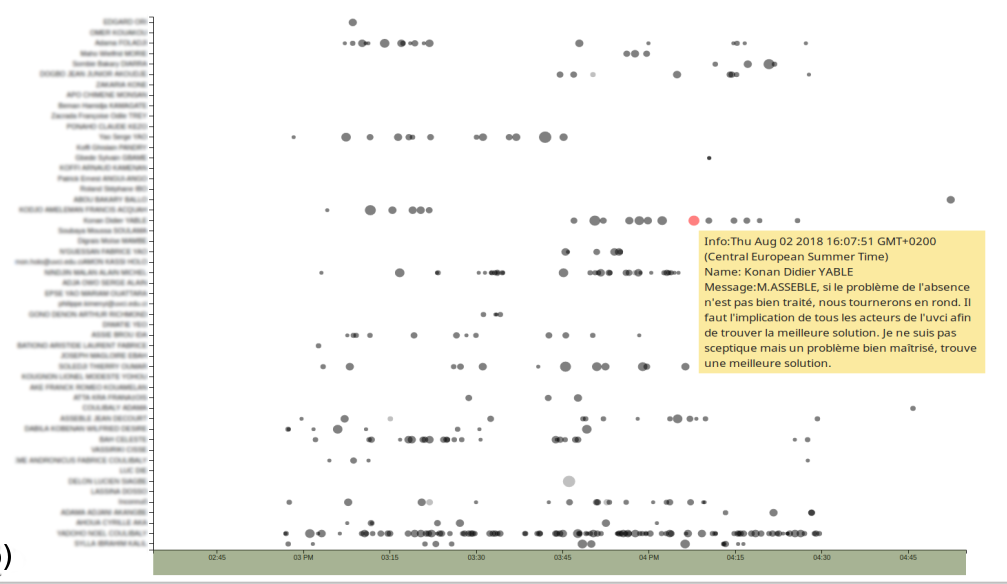
\includegraphics[width=.9\textwidth]{./Images/uvci_detail}}
    \end{block}
  }
  \only<6,7>{
    \only<6>{

      \begin{block}{multiplateform: Coursera}
        \centering
        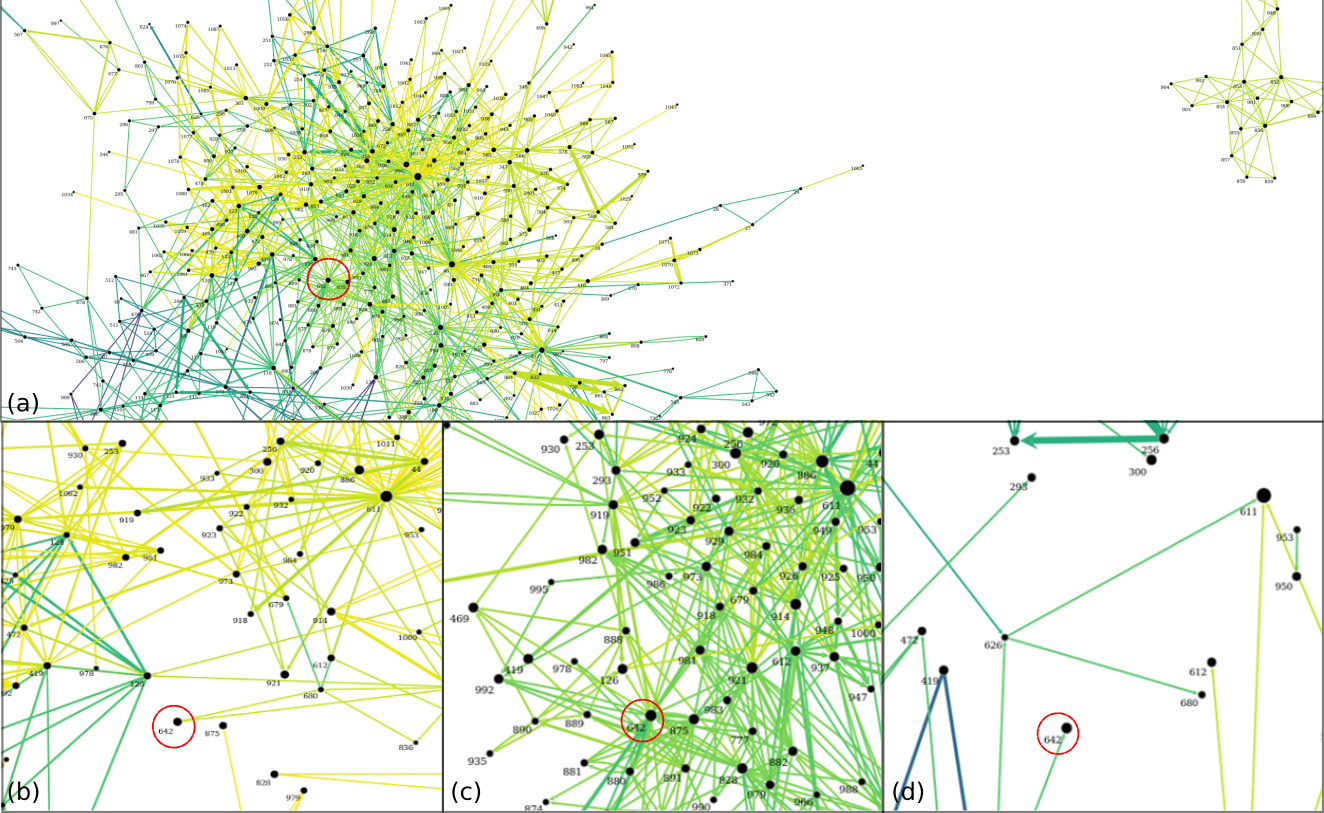
\includegraphics[width=.9\textwidth]{./Images/evolution}
      \end{block}
    }
    \only<7>{
      \begin{block}{multiplatform: Moodle}
        \centering
        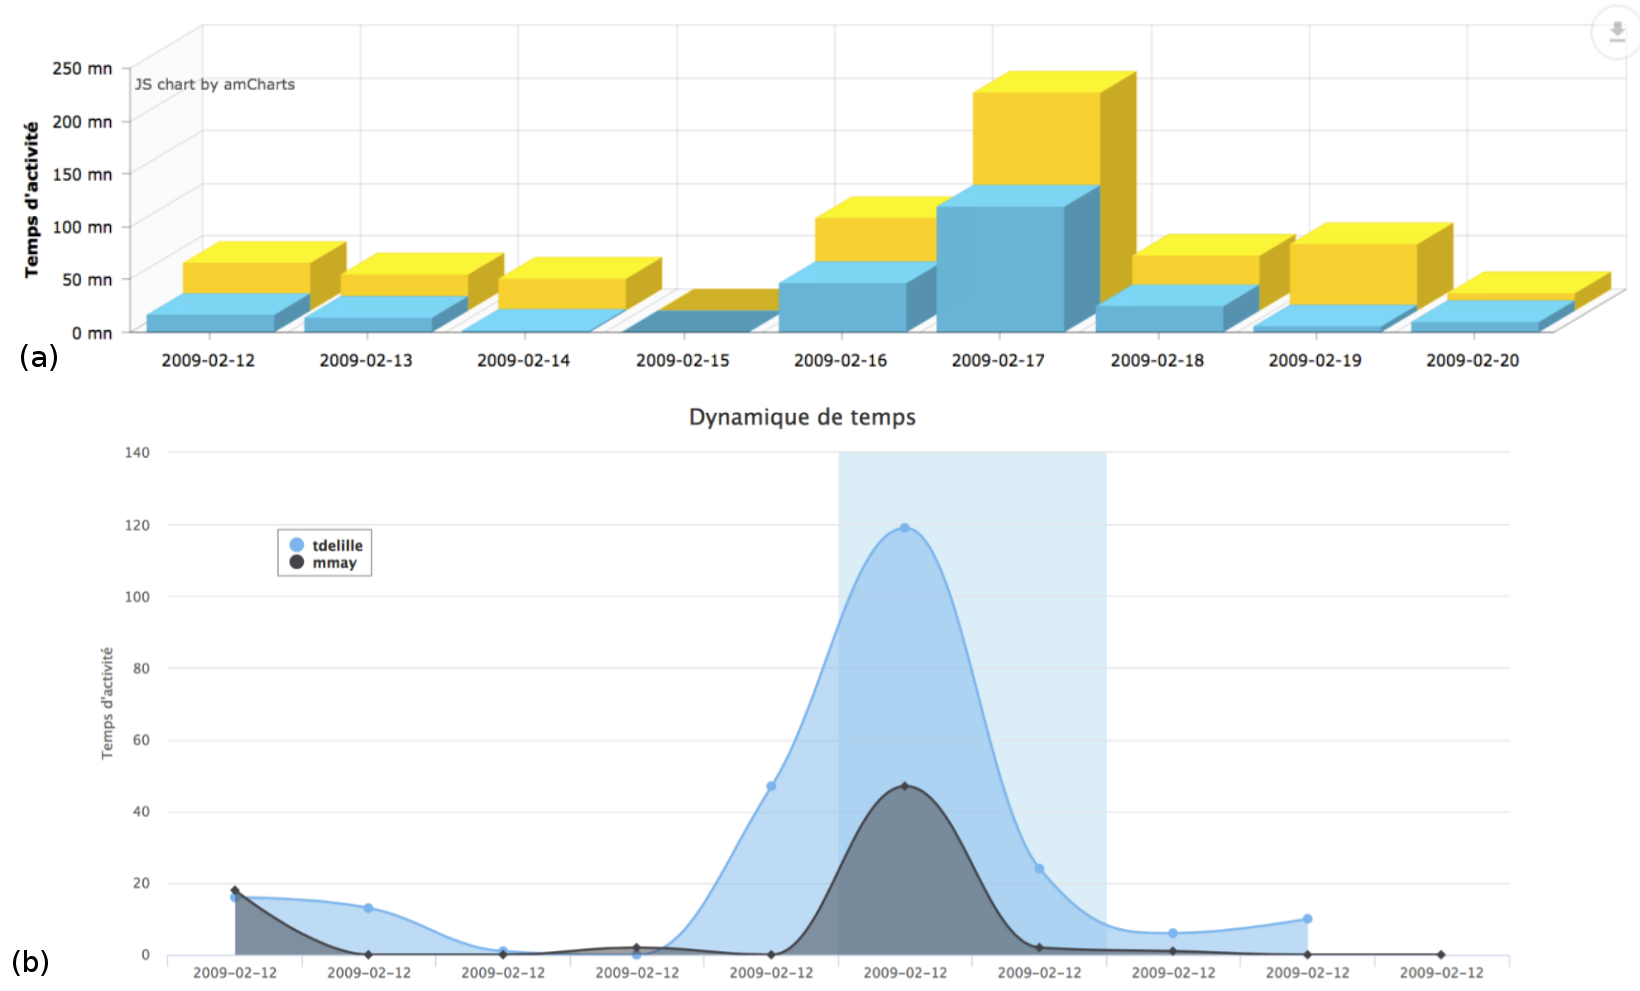
\includegraphics[width=.9\textwidth]{./Images/dynco_portrait}
      \end{block}
    }
  }
\end{frame}

\section{Conclusion and perspectives}
\begin{frame}{Section 5}
  \tableofcontents[sectionstyle=show/shaded,
  subsectionstyle=show/show/hide]
\end{frame}

\begin{frame}{We have}
  \begin{itemize}
  \item Explored ways to combine indicators in the three dimensions: temporal, structural and qualitative (NLP) to get a new indicator measuring collective dynamic
  \end{itemize}
  
  \begin{block}{Future perspectives are}
    \begin{itemize}
    \item to intergrate effectiveleny subjectif data
    \item to provide an usefull indicator for pedagogical conception
    \item to make sure the learning dashboard can be used in real time guidance
    \end{itemize}
  \end{block}
\end{frame}

\section{Biliography and thanks}
\begin{frame}[allowframebreaks]
  \Large \centering{ Towards visualizing collective dynamics in MOOC forums}
  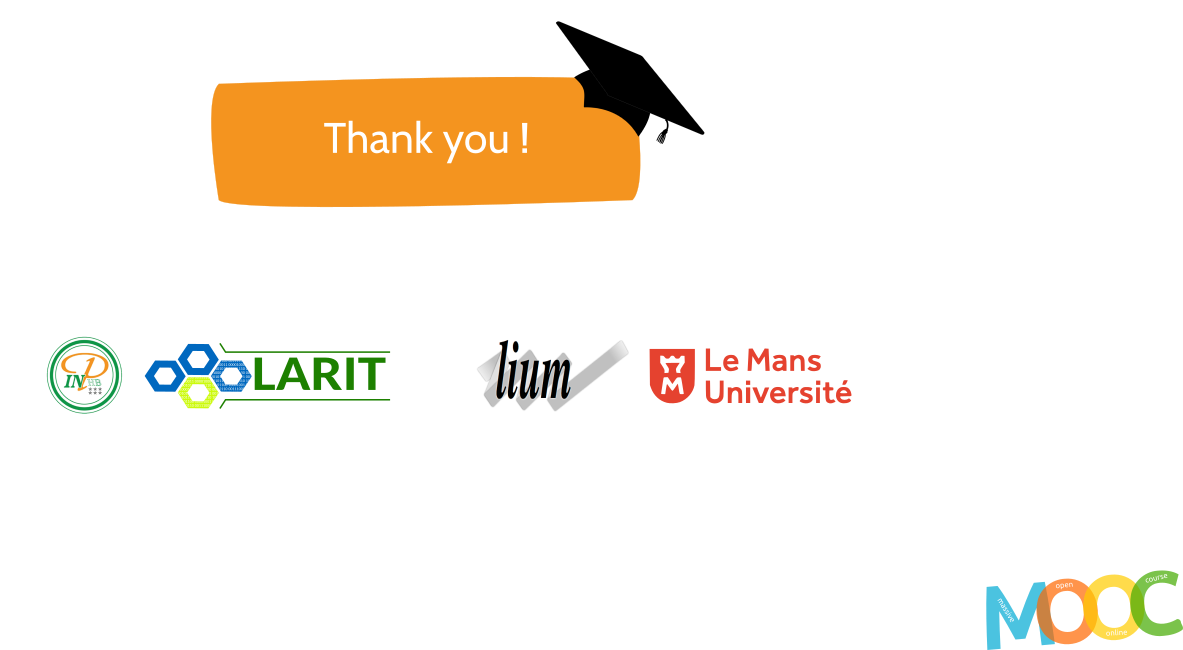
\includegraphics[width=\textwidth]{./Images/thanks}
\end{frame}
\end{document}